{\Large
\begin{center}
\textbf{КР №2 по экологии \\ ИУ7-63 \\	Фурдик Н.О. \\ Вариант 25 \\ ~\\Задание 1} \end{center}}
\begin{table}[h!]
	\caption{Сравнение ГЭС и ВЭС}
	\begin{tabular}{|p{4cm}|p{6cm}|p{6cm}|}
		\hline
		Характеристика  & ГЭС & ВЭС \\
		\hline
		Сложность строительства & Строительство ведётся только там, где есть большие запасы энергии воды, при этом стоит учитывать, что горные реки опасны из-за высокой сейсмичности районов. & Ветровые электростанции строят в местах с высокой средней скоростью ветра — от 4,5 м/с и выше. Предварительно проводят исследование потенциала местности. Анемометры устанавливают на высоте от 30 до 100 метров, и в течение одного—двух лет собирают информацию о скорости и направлении ветра. Скорость ветра возрастает с высотой. Поэтому ветровые электростанции строят на вершинах холмов или возвышенностей, а генераторы устанавливают на башнях высотой 30—60 метров.\\
		\hline
		Стоимость  & Ценность гидроэлектрической станции состоит в том, что для производства электрической энергии они используют возобновляемые природные ресурсы. В виду того, что потребности в дополнительном топливе для ГЭС нет, конечная стоимость получаемой электроэнергии значительно ниже, чем при использовании других видов электростанций. & Высокая стоимость оборудования. В результате это влияет и на цену конечного продукта - ветровой энергии. Говоря о финансовой стороне стоит упомянуть долгую и практически отсутствующую окупаемость оборудования. \\
		\hline
		КПД & 91-94\% & 33-35\% \\
		\hline
		Мощность & Самой мощной в России является Саяно-Шушенская ГЭС, установленная мощность - 6400МВт. В мире - 'Три ущелья', Китай; установленная мощность - 22 500 МВт. & Самой мощной в России является Адыгейская ВЭС, установленная мощность - 150МВт. В мире - 'Ганьсу', Китай; установленная мощность - 7965 МВт. \\
		\hline
		Сложность эксплуатации & У ГЭС можно выделить одно из главных преимуществ - простая эксплуатация. & Из-за сложности механизма ГЭС следует придерживаться немалого списка правил при эксплуатации. \\
		\hline
		
	\end{tabular}
\end{table}
\newpage
\begin{table}[h!]
	\begin{tabular}{|p{4cm}|p{6cm}|p{6cm}|}
		\hline
		Влияние на человека & Из минусов влияния на человека можно выделить разве что затопление пахотных земель. & Ветряные энергетические установки производят довольно много шума, в том числе сверхнизкий шум ветровых турбин (инфразвук), который не представляет опасности для человека в случае соблюдения разумного расстояния. \\
		\hline
		Влияние на экологию & Сокращённые и нерегулируемые попуски воды из водохранилищ по 10-15 дней (вплоть до их отсутствия) приводят к перестройке уникальных пойменных экосистем по всему руслу рек, как следствие, загрязнение рек, сокращение трофических цепей, снижение численности рыб, элиминация беспозвоночных водных животных,  повышение агрессивности компонентов гнуса (мошки) из-за недоедания на личиночных стадиях, а также сокращение потока биогенных веществ в океаны.& Для работы и генерации электричества ВЭС использую полностью экологически чистый источник - ветер. К тому же, ветропарк не наносит природе никакого урона, как, например, гидроэлектростанции. То есть, можно сказать, что ВЭС - экологически чистая и безвредная методика получения энергии. \\
		\hline
	\end{tabular}
\end{table}

\begin{center}
	\textbf{ГЭС Три ущелья} \end{center}
\begin{figure}[h!]
	\center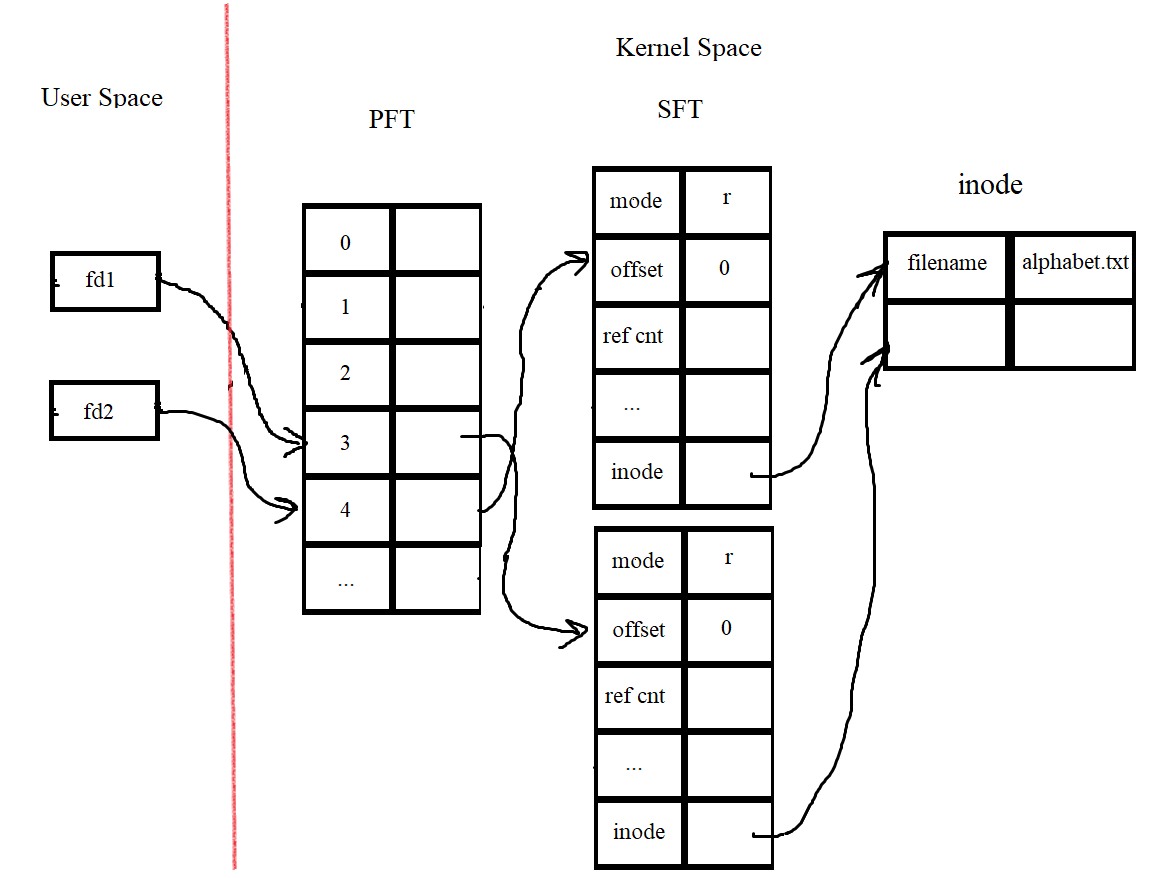
\includegraphics[scale=0.7]{2}
	\caption{ГЭС Три ущелья}
\end{figure}
\begin{enumerate}
	\item расположена на реке Янцзы в провинции Хубэй, Китай;
	\item установленная мощность - 	22500 МВт;
	\item номинальная мощность - 19750 МВт.
\end{enumerate}
\newpage
\begin{center}
	\textbf{Комплекс ВЭС Ганьсу} \end{center}
\begin{figure}[h!]
	\center
\includegraphics[scale=0.9]{1}
	\caption{Комплекс ВЭС Ганьсу}
\end{figure}
\begin{enumerate}
	\item расположен в провинции Ганьсу в городском округе Цзюцюань, КНР;
	\item установленная мощность - 7965 МВт;
	\item номинальная мощность - 6902 МВт.
\end{enumerate}

{\Large
	\begin{center}
		\textbf{Задание 2} \\ Недостаток чистой пресной воды\end{center}}
	
\begin{enumerate}
		\item Недостаток чистой пресной воды -- это отсутствие достаточных запасов водных ресурсов для удовлетворения потребностей населения,скота в чистой питьевой воде. Питьевая вода необходима для поддержания жизни и имеет первостепенное значение для человеческого здоровья. От дефицита питьевой воды страдает более 40\% мирового населения.
		 По данным счётчик аcountrymeters , население Земли на 25 апреля 2015 года достигло приблизительно 7 миллиардов 289 миллионов человек, а ежегодный прирост составляет примерно 83 миллионов человек. \cite {litlink1} Данные указывают на ежегодный прирост потребности в пресной воде в объёме 64 млн кубометров, в то время как общий объем воды на Земле составляет примерно 1400 млн куб. км, из которых лишь 2,5 \%, то есть около 35 млн куб. км, приходится на пресную воду.\cite {litlink2} Следует заметить, что за период времени, когда население планеты выросло в три раза, использование пресной воды возросло в 17 раз. Причём, по некоторым прогнозам, через 20 лет оно может увеличиться ещё втрое.
		 \item Дефицит питьевой воды связан с результатами изменения климата, с деятельностью человека, приводящей к сокращению водных ресурсов из-за загрязнения пресноводных экосистем, а также с последствиями урбанизации и изменений в землепользовании [3].
		 
		 По статистике, практически 1/5 часть мирового населения живёт в районах, в которых наблюдается серьёзная нехватка чистой питьевой воды. Кроме того, 1/4 населения живёт в развивающихся странах, которые испытывают нехватку из-за отсутствия инфраструктуры, необходимой для забора воды из водоносных пластов и рек.
		 
		 Одной из основных проблем является проблема загрязнения пресной воды, существенно снижающая уже существующие запасы. Этому загрязнению способствуют промышленные выбросы и стоки, смыв удобрений с полей, а также проникновение солёной воды в прибрежных зонах в водоносные слои из-за откачивания грунтовых вод.
		  \item Недостаток чистой воды вынуждает людей использовать для питья воду из небезопасных источников, которая опасна для здоровья. Потребление загрязнённой пресной воды приводит к ухудшению условий жизни, развитию заболеваний вплоть до смертельных исходов. Из-за нехватки воды существует практика хранения воды в жилищах, что существенно может повысить риск загрязнения и создания благоприятных условий для размножения вредных бактерий. Также, серьёзной является проблема гигиены. Люди не могут надлежащим образом мыться, стирать свою одежду и содержать в чистоте свои дома.\cite {litlink2}
		  
		  Если не предпринимать никаких мер, то к 2030 г. без удовлетворительной очистки воды будут оставаться почти 5 млрд человек, около 67 \% населения планеты. На сегодняшний день на каждого жителя Земли приходится около 750 м³ в год пресной воды, к 2050 г. это количество уменьшится до 450 куб. м. До 80 \% стран мира окажутся в зоне, которая по классификации ООН относится к категории ниже черты дефицита водных ресурсов. Только в Африке к 2020 г. из-за изменений климата в такой ситуации окажется от 75 до 250 млн человек. Нехватка воды в пустынных и полупустынных регионах вызовет интенсивную миграцию населения.\cite {litlink4}
		  \item Проблемам, связанным с водой, были посвящены Конференция ООН по водным ресурсам (1977 г.), Международное десятилетие снабжения питьевой водой и санитарии (1981—1990 гг.) \cite{litlink5}, Международная конференция по водным ресурсам и окружающей среде (1992 г.) и Всемирная встреча на высшем уровне «Планета Земля» (1992 г.).
		  
		  Для привлечения внимания мирового населения к проблеме нехватки пресной воды, 2003 г. был провозглашён Международным годом пресной воды. В том же году был учреждён механизм «ООН — водные ресурсы», который занимается вопросами, связанными с пресной водой и санитарией. Период 2005—2015 гг. Генеральная Ассамблея ООН провозгласила Международным десятилетием действий «Вода для жизни», координатором данной программы является механизм «ООН — водные ресурсы».
		  
		  Каждые три года Всемирная программа ООН по оценке водных ресурсов (WWAP) публикует Всемирный доклад ООН \cite{litlink6}, представляющий самую полную оценку состояния пресноводных ресурсов в мире.
		  \item В Египте воплощается в жизнь самый грандиозный из всех национальных проектов – “Тошка” или “Новая Долина”. Строительство продолжается уже на протяжении 5 лет и к 2017 году планируется завершение. Работы очень затратны для экономики страны, но перспективы представляются воистину глобальными. 10\% воды из Нила будет перенаправлено строящейся станцией в западные регионы страны, и площадь пригодной для жилья земли в Египте увеличится на целых 25\%. Более того, будут созданы 2,8 миллиона новых рабочих мест и более 16 миллионов человек будут переселены в новые проектируемые города. В случае удачи этого амбициозного проекта станет возможным повторный расцвет Египта как развитой державы с быстрорастущим населением.\cite {litlink4} \\Есть и другой пример активно развивающейся водной инфраструктуры при отсутствии собственных ресурсов. Различные пути борьбы с водным кризисом среди стран Персидского залива стали возможны с середины XX века благодаря нефтяному буму. Стали сооружаться дорогостоящие заводы по опреснению воды, и в результате на данный момент Саудовская Аравия и ОАЭ отличаются самыми солидными объёмами опреснения воды не только в регионе, но и в мире. По данным Arab News, Саудовская Аравия ежедневно использует 1,5 млн баррелей нефти на своих опреснительных установках, которые обеспечивают 50–70\% пресной воды в стране. В апреле 2014 г. в Саудовской Аравии открылся крупнейший в мире завод, производящий 1 млн куб. м воды и 2,6 тыс. МВт электроэнергии в сутки. Помимо этого, все страны Залива имеют развитые очистительные системы для утилизации и повторного использования загрязнённых вод. В среднем процент сбора сточных вод варьируется от 15\% до 70\% в зависимости от региона; самые высокие показатели (100\%) демонстрирует Бахрейн. Что касается использования очищенных сточных вод, то в этом лидируют Оман (100\% собранной воды используется повторно) и ОАЭ (89\%)\cite {litlink3}.
		  
		  По прогнозам, запасы пресной питьевой воды далеко не безграничны, и они уже подходят к концу. Согласно исследованиям, к 2025 году больше половины государств планеты либо ощутят серьёзную нехватку воды, либо почувствуют её недостаток, а к середине XXI века уже трём четвертям населения Земли не будет хватать пресной воды. По подсчётам, примерно в 2030 году 47\% населения планеты будут существовать под угрозой водного дефицита. При этом к 2050 г., значительно увеличится население развивающихся стран, в которых уже сегодня воды не хватает.
		  
		  С наибольшей вероятностью первыми останутся без воды Африка, Южная Азия, Ближний Восток и Северный Китай. По прогнозам, только в Африке к 2020 г. из-за изменений климата в данной ситуации окажется от 75 до 250 миллионов человек, а острая нехватка воды в пустынных и полупустынных регионах вызовет стремительную миграцию населения. Ожидается, что это коснётся от 24 до 700 миллионов человек.
		  
		  Среди стран-лидеров на данный момент предпринимается не так много усилий в этой области. Как это часто бывает, пока проблемы нет, кажется, что и не нужно уделять внимание факторам, могущим привести к её образованию. 
\end{enumerate}